%%
%% This is file `sample-sigconf.tex',
%% generated with the docstrip utility.
%%
%% The original source files were:
%%
%% samples.dtx  (with options: `sigconf')
%% 
%% IMPORTANT NOTICE:
%% 
%% For the copyright see the source file.
%% 
%% Any modified versions of this file must be renamed
%% with new filenames distinct from sample-sigconf.tex.
%% 
%% For distribution of the original source see the terms
%% for copying and modification in the file samples.dtx.
%% 
%% This generated file may be distributed as long as the
%% original source files, as listed above, are part of the
%% same distribution. (The sources need not necessarily be
%% in the same archive or directory.)
%%
%% Commands for TeXCount
%TC:macro \cite [option:text,text]
%TC:macro \citep [option:text,text]
%TC:macro \citet [option:text,text]
%TC:envir table 0 1
%TC:envir table* 0 1
%TC:envir tabular [ignore] word
%TC:envir displaymath 0 word
%TC:envir math 0 word
%TC:envir comment 0 0
%%
%%
%% The first command in your LaTeX source must be the \documentclass command.
\documentclass[sigconf]{acmart}
%% NOTE that a single column version may be required for 
%% submission and peer review. This can be done by changing
%% the \doucmentclass[...]{acmart} in this template to 
%% \documentclass[manuscript,screen]{acmart}
%% 
%% To ensure 100% compatibility, please check the white list of
%% approved LaTeX packages to be used with the Master Article Template at
%% https://www.acm.org/publications/taps/whitelist-of-latex-packages 
%% before creating your document. The white list page provides 
%% information on how to submit additional LaTeX packages for 
%% review and adoption.
%% Fonts used in the template cannot be substituted; margin 
%% adjustments are not allowed.
%%
%%
%% \BibTeX command to typeset BibTeX logo in the docs
\AtBeginDocument{%
  \providecommand\BibTeX{{%
    \normalfont B\kern-0.5em{\scshape i\kern-0.25em b}\kern-0.8em\TeX}}}

%% Rights management information.  This information is sent to you
%% when you complete the rights form.  These commands have SAMPLE
%% values in them; it is your responsibility as an author to replace
%% the commands and values with those provided to you when you
%% complete the rights form.
\setcopyright{acmcopyright}
\copyrightyear{2023}
\acmYear{2023}
\acmDOI{} %% isto

\usepackage{multirow}

%% These commands are for a PROCEEDINGS abstract or paper.
\acmConference[G53]{PRI}{December-10, 2023}{Porto, Portugal}
%
%  Uncomment \acmBooktitle if th title of the proceedings is different
%  from ``Proceedings of ...''!
%
%\acmBooktitle{Woodstock '18: ACM Symposium on Neural Gaze Detection,
%  June 03--05, 2018, Woodstock, NY} 
\acmPrice{15.00}
\acmISBN{978-1-4503-XXXX-X/18/06}


%%
%% Submission ID.
%% Use this when submitting an article to a sponsored event. You'll
%% receive a unique submission ID from the organizers
%% of the event, and this ID should be used as the parameter to this command.
%%\acmSubmissionID{123-A56-BU3}

%%
%% For managing citations, it is recommended to use bibliography
%% files in BibTeX format.
%%
%% You can then either use BibTeX with the ACM-Reference-Format style,
%% or BibLaTeX with the acmnumeric or acmauthoryear sytles, that include
%% support for advanced citation of software artefact from the
%% biblatex-software package, also separately available on CTAN.
%%
%% Look at the sample-*-biblatex.tex files for templates showcasing
%% the biblatex styles.
%%

%%
%% The majority of ACM publications use numbered citations and
%% references.  The command \citestyle{authoryear} switches to the
%% "author year" style.
%%
%% If you are preparing content for an event
%% sponsored by ACM SIGGRAPH, you must use the "author year" style of
%% citations and references.
%% Uncommenting
%% the next command will enable that style.
%%\citestyle{acmauthoryear}

%%
%% end of the preamble, start of the body of the document source.
\begin{document}

%%
%% The "title" command has an optional parameter,
%% allowing the author to define a "short title" to be used in page headers.
\title{Privago: Hotels Search System based on their reviews}

%%
%% The "author" command and its associated commands are used to define
%% the authors and their affiliations.
%% Of note is the shared affiliation of the first two authors, and the
%% "authornote" and "authornotemark" commands
%% used to denote shared contribution to the research.
\author{André Costa}
\email{up201905916@edu.fe.up.pt}
\affiliation{%
  \institution{Faculty of Engineering - University of Porto}
  \city{Porto}
  \country{Portugal}
}

\author{André Ávila}
\email{up202006767@edu.fe.up.pt}
\affiliation{%
  \institution{Faculty of Engineering - University of Porto}
  \city{Porto}
  \country{Portugal}
}

\author{Fábio Sá}
\email{up202007658@edu.fe.up.pt}
\affiliation{%
  \institution{Faculty of Engineering - University of Porto}
  \city{Porto}
  \country{Portugal}
}

\author{Fábio Morais}
\email{up202008052@edu.fe.up.pt}
\affiliation{%
  \institution{Faculty of Engineering - University of Porto}
  \city{Porto}
  \country{Portugal}
}


%%
%% The abstract is a short summary of the work to be presented in the
%% article.
\begin{abstract}
The internet's rapid growth demands appropriate systems for harnessing and connecting this massive information resource. This project addresses this need by focusing on the hotel industry, where reviews play a crucial role in shaping consumer choices. This article aims to provide a clear and well-documented explanation of the work needed in developing a robust search engine for hotel reviews. To accomplish this, data is collected from four different Kaggle datasets, cleaned and prepared, and in-depth data analysis is undertaken, as we seek to fulfill prospective search tasks such as finding hotels near the airport or finding hotels with a helpful staff. The data is then transformed into a collection on Apache Solr's search engine, where it undergoes analysis and refinement through manipulation of various characteristics.

The project achieved significant milestones. The 'Data Preparation' phase successfully navigated challenges, creating a finalized dataset that balances data richness and relevance. The 'Information Retrieval' phase executed planned tasks, overcoming challenges in handling nested documents. Evaluation confirmed the system's stability and capability to address various information needs. The 'Information Retrieval Improvement' phase concluded, implementing targets such as applying the Stop Words filter for common word sensitivity and testing sentimental semantic analysis. Additionally, user interface enhancements have been successfully introduced, providing a more intuitive and user-friendly experience. This refined hotel search engine now empowers travelers with improved tools to filter accommodations based on preferences identified during the analysis phase.
\end{abstract}

%%
%% The code below is generated by the tool at http://dl.acm.org/ccs.cfm.
%% Please copy and paste the code instead of the example below.
%%
\begin{CCSXML}
<ccs2012>
<concept>
<concept_id>10002951.10003317.10003325</concept_id>
<concept_desc>Information systems~Information retrieval query processing</concept_desc>
<concept_significance>100</concept_significance>
</concept>
</ccs2012>
\end{CCSXML}

\ccsdesc[100]{Information systems~Information retrieval query processing}


%%
%% Keywords. The author(s) should pick words that accurately describe
%% the work being presented. Separate the keywords with commas.
\keywords{Hotels, Reviews, Information, Dataset, Data Retrieval, Data Preparation, Data Analysis, Data Processing, Data Refinement, Pipeline, Data Domain Conceptual Model, Information Retrieval
}


%%
%% This command processes the author and affiliation and title
%% information and builds the first part of the formatted document.
\maketitle

\section{Introduction}


The choice of the hotel reviews theme is motivated by the large amount of information's sources and the rich diversity of attributes it encompasses. Hotel reviews, as a research focus, hold substantial importance in the modern information landscape. They not only provide valuable insights into the hospitality industry but also serve as a prime example of data diversity, combining numerical rates, submission dates, and personal, subjective narratives. This diversity introduces intricacies in data structuring and presents challenges in contextual search, making it an ideal choice for aligning the search system with real-world scenarios. Thus emphasizing practical applicability and the development of robust information retrieval solutions.

This document is structured into several major sections. We commence with \textbf{Data Extraction and Enrichment}, where we introduce the data sources, briefly characterize the datasets, and assess data quality. Subsequently, \textbf{Data Preparation} outlines the selection criteria, processing methods, and data storage procedures for hotel-related information and associated reviews, following a clear and reproducible pipeline.

In \textbf{Data Characterization} we delve into the evaluation and visualization of the refined data. This involves examining various criteria and relationships, from the Domain Conceptual Model to Word Clouds.

\textbf{Possible Search Tasks} provide an overreaching interpretation of the results, guiding the identification of suitable research objectives for the \textbf{Information Retrieval}, where the documents are indexed and searched using Apache Solr \cite{Apache_Solr} with a defined schema and defined parameters. Finally, the \textbf{Evaluation} analyses the results obtained by custom queries on the prepared search engine, which was defined on the previous section.

\section{Data Extraction and Enrichment}

After conducting research for relevant data in terms of variety and quantity, four datasets in CSV format from different regions were selected through the Kaggle \cite{kaggle} platform. Table ~\ref{tab:initFreq} provides a characterization of the acquired datasets:

\begin{table}[h]
\small
\caption{Initial datasets characterization}
\label{tab:initFreq}
\begin{tabular}{lllll}
\toprule
Dataset & Features & Hotels & Reviews & Size(MBs)\\
\midrule
Datafiniti's Hotel Reviews & 26 & 1400 & 10000 & 124.45 \\
Hotel Review Insights & 7 & 570 & 7000 & 1.31 \\
London Hotel Reviews & 6 & 20 & 27329 & 22.85 \\
Europe Hotel Reviews & 17 & 1493 & 515000 & 238.15 \\
\bottomrule
\end{tabular}
\end{table}


The Datafiniti's Hotel Reviews \cite{Datafiniti's_Hotel_Reviews} dataset was taken from Datafiniti's Business Database \cite{Datafiniti's_Business_Database} through sampling. Hotel Review Insights \cite{Hotel_Review_Insights} is a compilation of hotels around the world through web-scraping of reviews found on Booking.com \cite{Booking}. London Hotel Reviews \cite{London_Hotel_Reviews} is a sample taken and partially refined from a DataStock dataset \cite{DataStock}. Finally, Europe Hotel Reviews \cite{Europe_Hotel_Reviews} also results from web scrapping of hotel reviews across Europe published on Booking.com \cite{Booking}.

%% Figure 9
\begin{figure}[H]
  \centering
  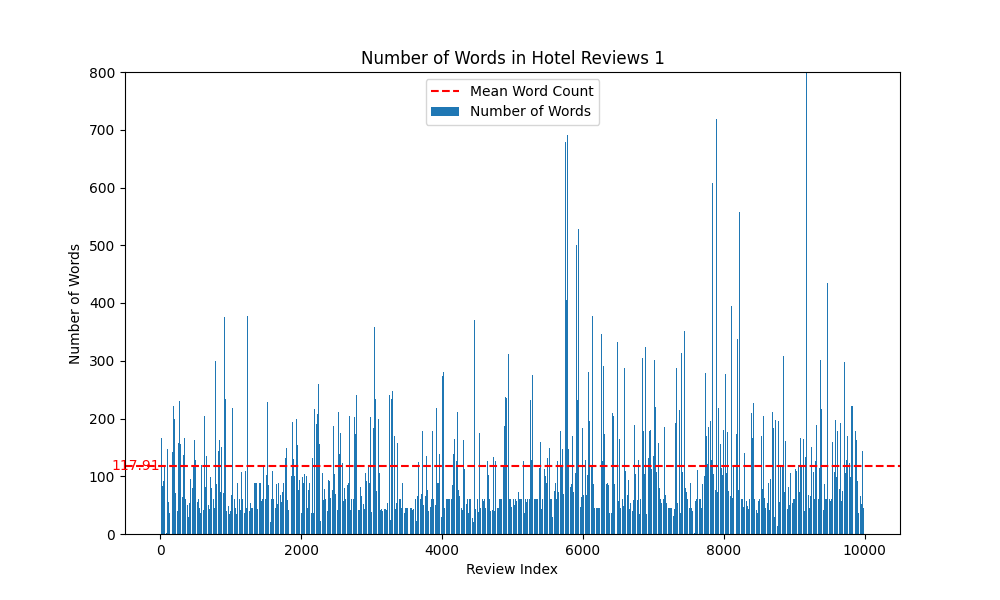
\includegraphics[width=\linewidth]{imgs/word_count_1.png}
  \caption{Average words per review in Datafiniti's Hotel Reviews dataset}
  \label{fig:reviewWords1}
\end{figure}

All datasets have a public use license and, according to the Kaggle platform, a usability index greater than 8. This index is justified, given that the elimination of null, repeated or non-informative entries practically did not eliminate nothing.

The datasets contain common features, numerical data, such as rate, review date, and textual data, such as review text, hotel location and name. The last dataset contains two additional parameters, positive review and negative review. The features stated were extracted in this step and refined in Data Preparation.


\section{Data Preparation}

In this section, is presented the structured data preparation pipeline [~\ref{fig:pipeline}] that was developed for the project. This pipeline embrace various data cleaning and restructuring procedures aimed at achieving a clean, uniform, and ready to analyze dataset. The goal of this stage is to build a strong basis for insightful analysis.

The data preparation process began with a comprehensive cleaning phase, where the primarly focus was the removal of records containing \textbf{empty or null values} in any attribute. Simultaneously, was identified and eliminated incomplete or uninformative data, including strings with \textbf{uninformative text}, such as "no comments available for this review.", using Python. This combined cleaning step ensured that the dataset was cleansed in detail for the normalization phase.

With the data cleaned, attention was turned to \textbf{attribute normalization}. Given the presence of diverse datasets with varying formats, comprehensive normalization process was needed. This included standardizing attributes such as \textbf{"positive\_reviews"} and \textbf{"negative\_reviews"} into a unified \textbf{"review\_text"} attribute for the 4th dataset as is demonstrated in the Pipeline Diagram [Figure ~\ref{fig:pipeline}]. Additionally, \textbf{date formats} were normalized to ensure uniformity and suitability for analysis. The date format was set as "year-month" due to the absence of day-specific review information in the second dataset and its irrelevance to the research targets.\textbf{Rate scales} were also normalized to a common range and converted to floating-point values, facilitating comparative analysis ([0.0, 5.0]).

In addition, was established a \textbf{standardized naming} convention to address variations in \textbf{hotel names}, such as from \textit{"45 Park Lane - Dorchester Collection"} to \textit{"45 Park Lane Dorchester Collection"}. This step was necessary to facilitate the aggregation step and the addition of the feature "average\_rate" to each hotel entity, referenced below. \textbf{Location standardization} involved reducing location names to their last two words, preserving only the capital and country names.

To gain insights into the textual content, we calculated the temporary column \textbf{word count} for each review across all datasets. This analysis was facilitated using the Pandas \cite{Pandas} Python tool, allowing us to extract valuable information such as quartile ranges and make informed decisions during the review deletion phase. This process enabled us to identify and manage reviews with either an insufficient word count or an excessively high word count. We achieved this by removing reviews falling below the 25\% threshold (first quartile) and those exceeding the 75\% threshold (fourth quartile). This step was done separately for each dataset, due to the discrepation of each average word counting [Figure ~\ref{fig:reviewWords1}] [Figure ~\ref{fig:reviewWords3}].

At this stage, all the datasets were successfully merged into a single, consolidated dataset, which streamlined the remaining preparation tasks. These tasks commenced with the computation of the temporary column \textbf{"average\_rate"} for each unique hotel. This information may prove valuable for defining search criteria in future milestones.

After completing the aforementioned steps, the next phase involved determining the minimum and maximum number of \textbf{reviews per hotel} to be retained. To accomplish this, the same approach used for analyzing the number of words per review was employed, utilizing the Pandas \cite{Pandas} .describe() function. This statistical analysis provided essential insights into the distribution of reviews across hotels. This step was important due to the discrepation of the number of reviews per hotel [Figure ~\ref{fig:reviewsHotel}].

%% Figure 11
\begin{figure}[H]
  \centering
  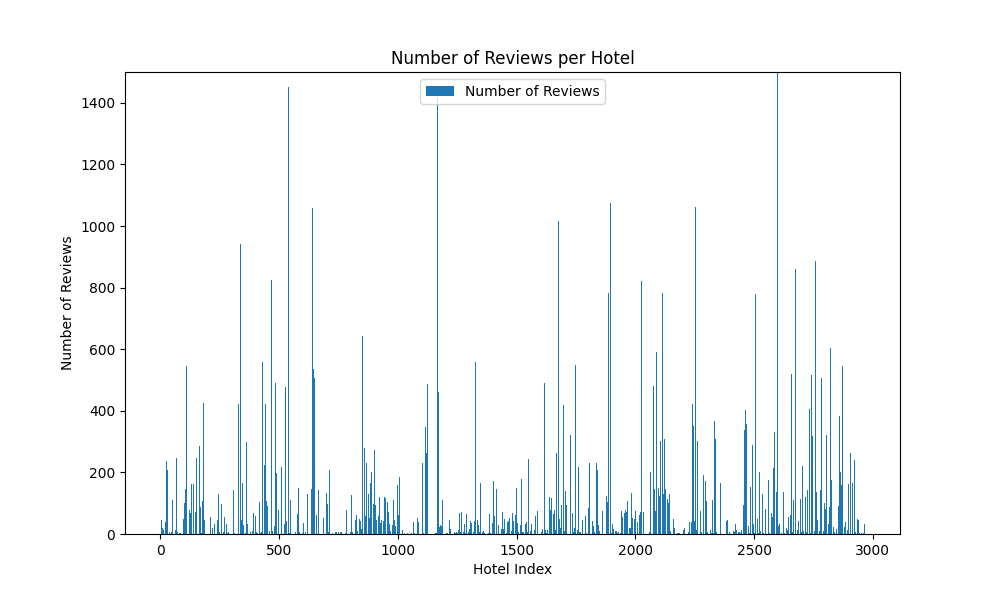
\includegraphics[width=\linewidth]{imgs/hotel_reviews_number.png}
  \caption{Number of Reviews per Hotel}
  \label{fig:reviewsHotel}
\end{figure}

First, hotels with fewer reviews, falling below the established minimum threshold (first quartile), were addressed, and they were subsequently removed from the dataset. This step was crucial in ensuring that the dataset focused exclusively on hotels with a volume of reviews contained in the second and third quartile, thus providing more meaningful insights.

Subsequently, hotels with an excessive number of reviews were taken into account. To handle this situation, a strategy was implemented, allowing the selection and retention of reviews while preserving the proportion of reviews per rate category for each specific hotel, i.e., its global rate. This approach guaranteed a balance between the "average\_rate" and the rate of the selected reviews.

The final step in the data preparation phase involved organizing the data into the \textbf{desired JSON file format}, which was designed based on our UML diagram [Figure ~\ref{fig:uml}] and with a focus on the primary objective of the search tool. This format consisted of a collection of JSON objects, each representing a "Hotel" entity. Within each "Hotel" object, were included not only its associated attributes (name, location, average\_rate) but also the related reviews, presented as JSON objects themselves. Each review has a corresponding text, rate and submission date.

\section{Data Characterization}

In this section there is a characterization of the documents that are produced by the pipeline. The graphs and tables were obtained using the Matplotlib \cite{Matplotlib}, Numpy \cite{Numpy} and NLTK \cite{NLTK} libraries.



\begin{figure}[h]
  \centering
  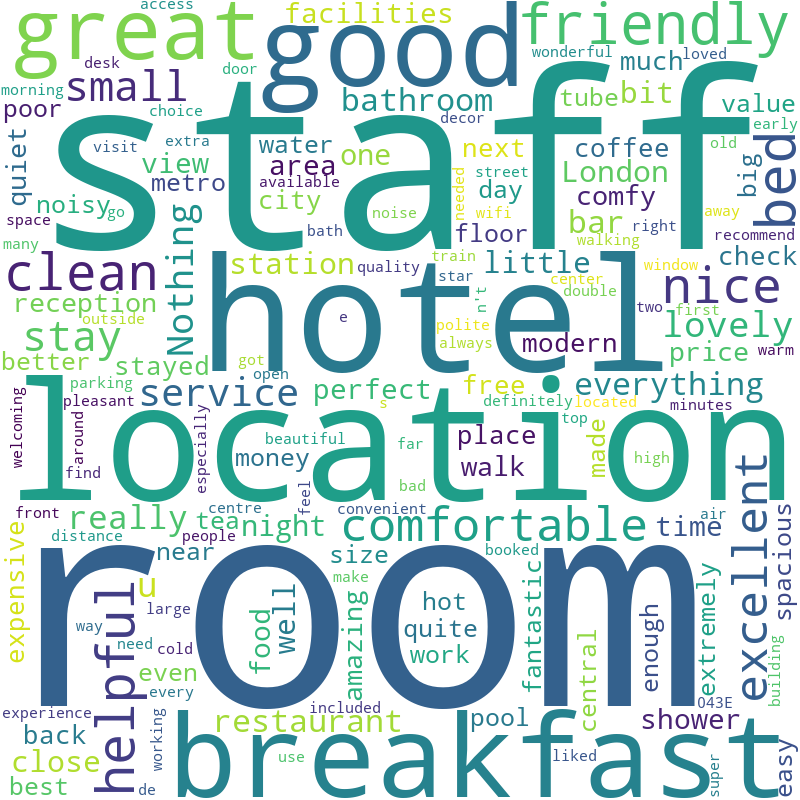
\includegraphics[width=\linewidth]{imgs/reviews_wordcloud.png}
  \caption{Reviews Word Cloud}
  \Description{TODO}
  \label{fig:wordcloud}
\end{figure}

The word cloud based on the texts of the reviews supports the search tasks of the next milestone as well as the contextual search to be implemented. As expected, the words that stand out the most are those intrinsically related to the hotel industry, such as "staff", "room", "location", "breakfast". Generally, the highlighted words have a neutral tone, although several with a very positive connotation are also detectable, such as "clean", "great", "lovely", "excellent", which can also be proven by the average rate [Figure ~\ref{fig:averageRateDistribution}] given to hotels.

\begin{figure}[h]
  \centering
  \includegraphics[width=\linewidth]{imgs/top_locations.png}
  \caption{Hotel location distribution}
  \Description{TODO}
  \label{fig:hotelLocationDistribution}
\end{figure}


Figure [~\ref{fig:hotelLocationDistribution}] shows the distribution of the 10 most frequent hotel locations in the system. As expected, the capitals and large cities of the main tourism countries concentrate the largest number of hotels and their reviews.



As we can see in figure [~\ref{fig:averageRateDistribution}] Hotels tend to have very good reviews. The result is encouraged by their locations, as the majority are in cities with major tourist attractions and therefore with a greater cadence of reviews.

\begin{figure}[H]
  \centering
  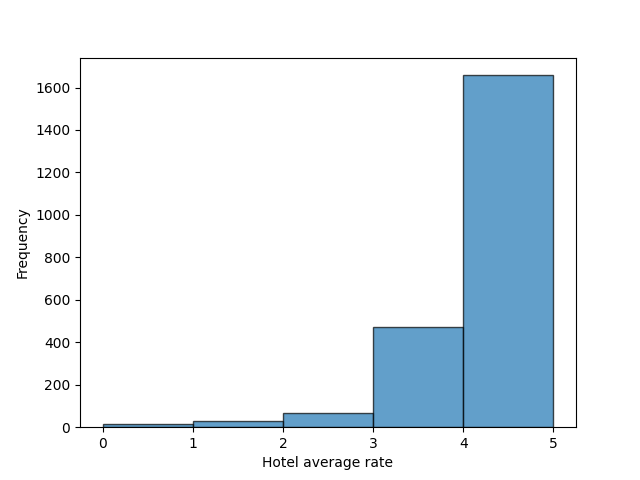
\includegraphics[width=\linewidth]{imgs/rating_distributions.png}
  \caption{Average rate distribution}
  \Description{TODO}
  \label{fig:averageRateDistribution}
\end{figure}

From the analysis of the figure [~\ref{fig:reviewsDistributionYear}], it can be concluded that the system includes hotels with reviews from 2010 to 2023. However, the choice of initial datasets with information relating mainly to the period 2015 and 2017 influenced their representativeness.

%% Figure 7
\begin{figure}[H]
  \centering
  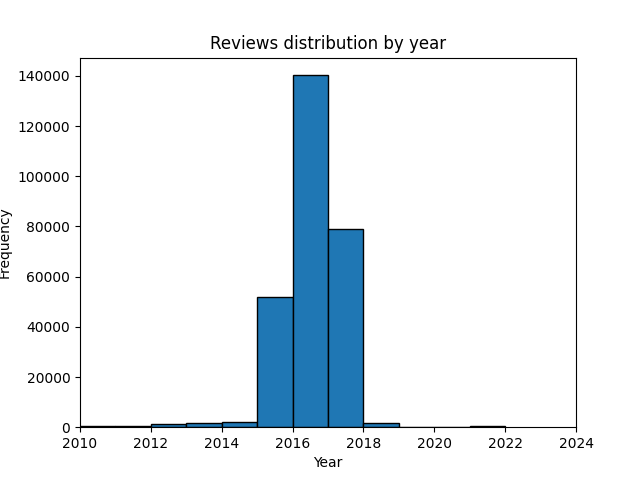
\includegraphics[width=\linewidth]{imgs/date_distributions.png}
  \caption{Reviews distribution per year}
  \Description{TODO}
  \label{fig:reviewsDistributionYear}
\end{figure}

Let's look, for example, at the distribution of reviews by month in 2016 in the figure [~\ref{fig:monthsDistribution}].

%% Figure 8
\begin{figure}[H]
  \centering
  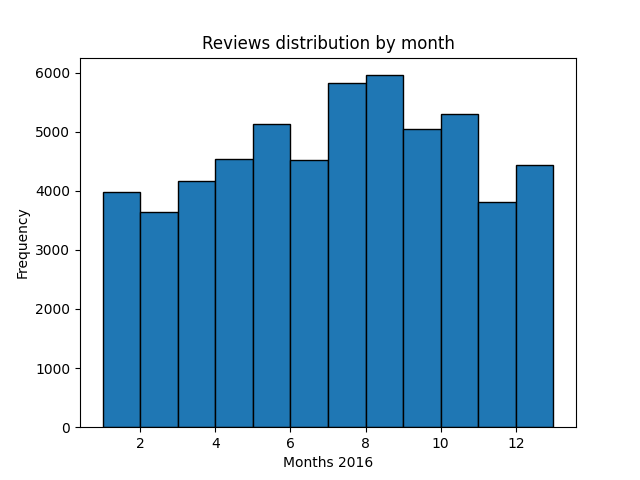
\includegraphics[width=\linewidth]{imgs/date_distributions_2016.png}
  \caption{Month reviews distribution in year 2016}
  \Description{The figure shows a bar chart, the bars represent the frequency (y axis) for every month (x axis of the year), its values range from around 3750 to 6000, the chart shows an increase in frequency in the first nine months (reaching the highest value of around 6000) with exception for the second month (which has the lowest value of the chart with 3750), then there is a decrease in frequency for the last four months with the odd numbered months having slightly higher values than their previous month. }
  \label{fig:monthsDistribution}
\end{figure}

As we can see, it is July and August when the number of reviews is higher. This period corresponds to the Summer time when people normally take vacations and therefore choose to travel. This pattern is repeated for the other years under analysis.

\subsection{Data Conceptual Model}

After the Data preparation phase, our documents contain the following relationships:

\begin{figure}[H]
  \centering
  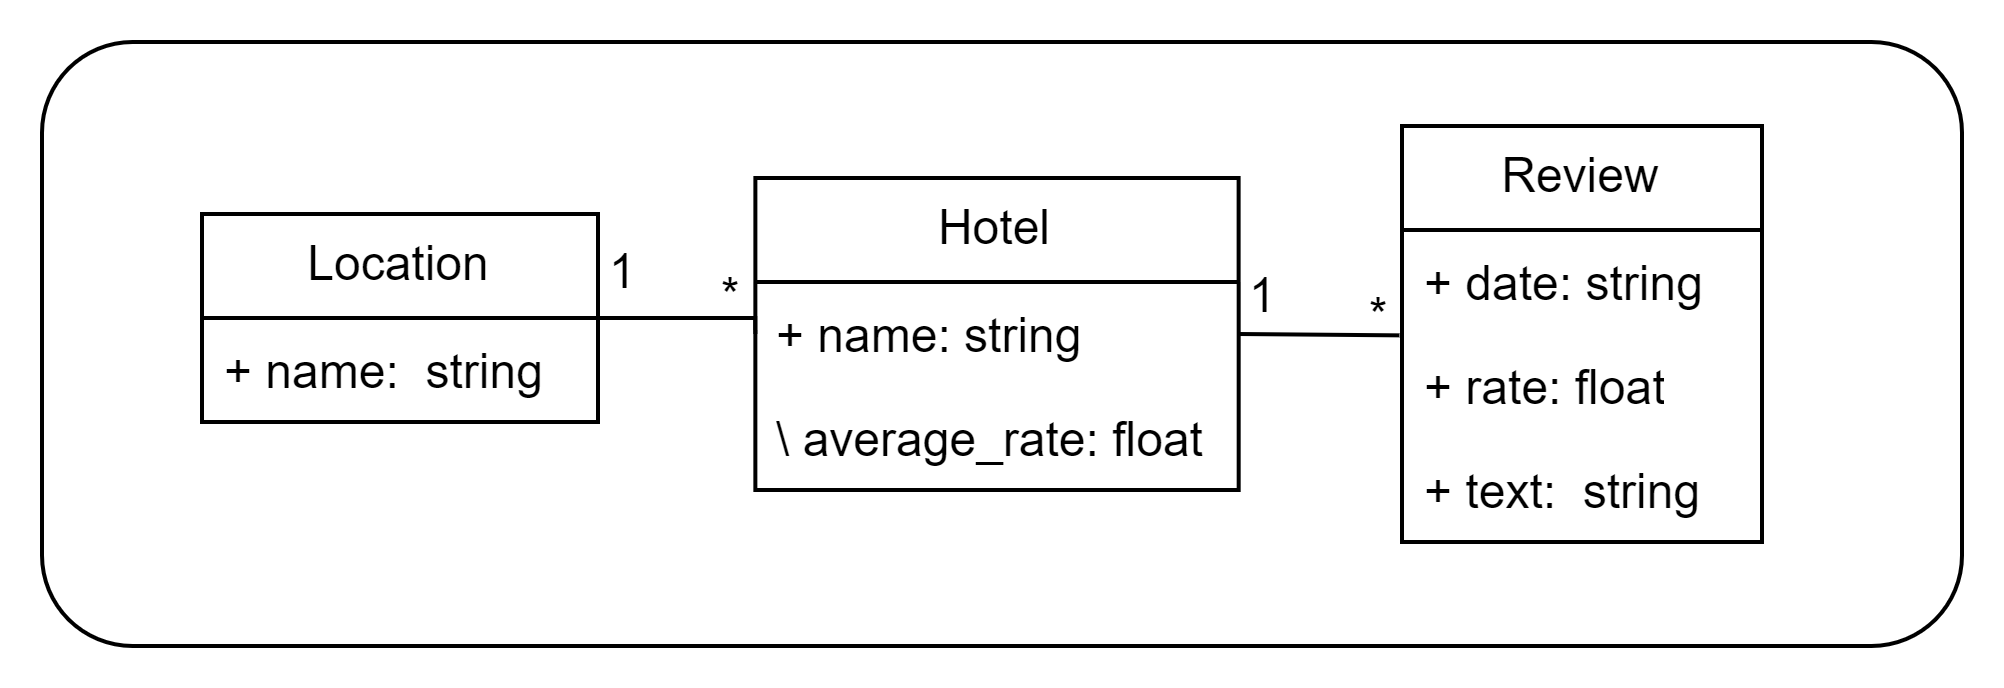
\includegraphics[width=\linewidth]{imgs/UML.png}
  \caption{Data Conceptual Model}
  \Description{TODO}
  \label{fig:uml}
\end{figure}

A hotel is made up of the attributes name, location and average\_rate. Note that average\_rate is a derived attribute that was calculated in the process based on the selected reviews. Each review has the corresponding text, rate and submission date.

Location was also considered a class because, as expected in the hotel scene, there are several hotels per region, mainly in large cities, as shown in figure [~\ref{fig:hotelLocationDistribution}].


\section{Possible search tasks}

In the course of the data analysis journey, were unveiled valuable insights through the use of a Word Cloud Diagram [Figure ~\ref{fig:wordcloud}]. This visual representation highlighted the most frequently occurring words in hotel reviews, shedding light on what matters most to travelers. Among these words, some stood out as pivotal in understanding the key factors that influence hotel choice and guest satisfaction.

\textbf{"Location"} emerged as one of the top considerations in travelers' decision-making processes. Whether it's proximity to local attractions, accessibility to transportation hubs, or the overall neighborhood ambiance, the location of a hotel can greatly influence the overall travel experience. Search scenarios such as \textbf{"Hotel in the United Kingdom with good location and either elevator or good accessibility."} and \textbf{"The best hotels near center of London."} can help travelers selecting accommodations that align with their preferred locations and provide convenient access to their destinations.

The words "breakfast" and "service" had a prominent presence in the word cloud [Figure ~\ref{fig:wordcloud}], suggesting a keen interest in this aspects. Whether it's a hearty breakfast buffet or unique morning options, travelers seek accommodations that cater to their breakfast preferences. Another one of the foremost considerations in hotel selection is the quality of the room and its amenities. Words like "room," "bed," and "bathroom" featured prominently in our Word Cloud [Figure ~\ref{fig:wordcloud}], underscoring the importance of these aspects to travelers. Searches related to "room"/"bed" quality or "bathroom" sanitation can guide travelers to accommodations that prioritize comfort and cleanliness. A search such as \textbf{"Hotels with good breakfast or good room service in New Delhi"} could be instrumental in identifying hotels that excel in the breakfast provided or in the room service available to their guests.

The context about the hotels left in their reviews adds the possibility of searching for specific details, for example, a person that follows a vegetarian diet might be struggling to find compatible hotels, this hassle could be resolved with a search such as \textbf{"Hotels with good vegetarian/vegan options"}.

\section{ Information Retrieval}

Information Retrieval \cite{Information_Retrieval} is the process of finding and extracting relevant information from large collections of naturally unstructured data, such as texts. This extraction is based on documents, which are the result of restructuring the initial data, and the output is sorted by relevance, becoming the main challenge.

This section presents the indexing and query methods used in this information retrieval system powered by previously constructed documents. 

The implementation of the search system is based on Apache Solr \cite{Apache_Solr} , an open-source tool that offers various features relevant to the project's purpose, including distributed and fast indexing, scalability, and advanced search capabilities surpassing a full-text match.

\subsection{Document Characterization}

The documents to be indexed and searched in the system are those resulting from the processes of data extraction, enrichment, and aggregation in the pipeline described above.

Therefore, a hotel is a document consisting of a name, average rating, location, and has a set of associated reviews. These reviews have their corresponding date, the assigned rating, and the user's comment about the hotel.

\subsection{ Indexing Process}

Indexing serves as a fundamental step in Information Retrieval, optimizing search efficiency by organizing the data. It involves creating a structured index that enhances both search speed and scalability. Without proper indexing, search systems would face challenges, resulting in slower response times and increased computational overhead.

In Solr, various types of indexing exist for document fields and associated queries, based on a Tokenizer \cite{Solr_Tokenizers} and Filters \cite{Solr_Filters}. While Tokenizers create a token stream from the original string following a predefined rule, Filters transform these tokens for consistency in subsequent searches and matches.
    
In this specific case, the focus was primarily on indexing textual fields, as they provide the most context and information for searches. Conversely, given the project's context, it is not expected to search for specific dates or review ratings. Therefore, these latter two document fields were not indexed.

Textual fields were indexed by instantiating a new data type. The \textbf{`boosted\_text`} index analyzer includes:

\begin{itemize}
    \item \textbf{\textit{StandardTokenizerFactory}} tokenizer: splits texts based on punctuation and spaces; 
    \item \textbf{\textit{ASCIIFoldingFilterFactory}} filter: handles special characters and accents, converting them to their equivalent ASCII form;
    \item \textbf{\textit{LowerCaseFilterFactory}} filter: converts all characters to their lowercase counterparts;
    \item \textbf{\textit{SynonymGraphFilterFactory}} filter: expands each token to include variations based on its synonyms;
    \item \textbf{\textit{EnglishMinimalStemFilterFactory}} filter: reduces each token to its root form, facilitating the search for variations of specific terms;
\end{itemize}

Fields with native values were defined using Solr's default types. The English language was chosen for both stem assignment and synonym generation, aligning with the language of the manipulated data.

The \textbf{SynonymGraphFilterFactory} is crucial in this context. Since the search is conducted based on reviews, which are inherently subjective, derived from natural language and rich in adjectives, it is important not to rely on specific terms but rather to match synonyms of terms.

The same structure was used for the query analyzer. Thus, the indexing of the final document can be characterized by the following schema:

\begin{table}[H]
\caption{Schema Field Types}
\label{tab:schema_types}
\begin{tabular}{lll}
\toprule
Field & Type & Indexed\\
\midrule
name & boosted\_text & yes\\
location & boosted\_text & yes\\
average\_rate & pdoubles & yes\\
date & string & no \\
rate & pdoubles & no \\
text & boosted\_text & yes \\
\bottomrule
\end{tabular}
\end{table}

\subsection{Retrieval Process and Setup}

The approach implemented involves two schemas: a simple schema utilizes default field types for each field, while the more complex schema incorporates instantiated field types for enhanced search capabilities. 

For query parameters used by both schemas, the system incorporates the following:
\begin{itemize}
    \item \textbf{Query (\texttt{q})}: Focuses on the most valuable words in the query.
    \item \textbf{Query Operator (\texttt{q.op})}: Utilizes OR $|$ AND for query operations.
    \item \textbf{Query Filter (\texttt{fq})}: Defines a query that can be used to restrict the superset of documents.
    \item \textbf{Filter List (\texttt{fl})}: Limits the information included in a query response.
    \item \textbf{Sort Field (\texttt{sort})}: Specifies the sorting value for the results.
\end{itemize}

\begin{table}[h]
\caption{Query parameters}
\label{tab:query_params}
\begin{tabular}{ll}
\toprule
Parameter & Value\\
\midrule
q & (strong wifi)  \\
q.op & AND \\
fq & {!child of="*:* - \_nest\_path\_:*"} location: "New York" \\
fl & *,[child] \\
sort & score desc \\
\bottomrule
\end{tabular}
\end{table}

The need of the fl and fq parameters results from the inclusion of nested documents \cite{Indexing_Nested} \cite{Queries_Nested} . The final dataset consists of hotels, each containing a list of reviews. Recognizing the relevance of both hotels and reviews as distinct documents, a distinct approach to the search process was necessary. The combined use of fl and fq proved to be efficient in this step.

Additional query criteria the simple schema uses the default type, while the boosted schema employs the type created by eDismax \cite{eDismax} with specific parameters for optimizing search engine results:

\begin{itemize}
    \item \textbf{Query Field with Optional Boost (\texttt{qf})}: This assigns weights to specific fields in the search;
    \item \textbf{Phrase-Boosted Field (\texttt{pf})}: Focuses on selecting more relevant terms from the query;
    \item \textbf{Phrase Boost Slope (\texttt{ps})}: Defines the maximum number of tokens between searched words;
\end{itemize}

\begin{table}[H]
\small
\caption{defType eDismax parameters}
\label{tab:edismax_par}
\begin{tabular}{ll}
\toprule
Parameter & Value\\
\midrule
qf & text\textasciicircum{} 7 name location\textasciicircum{}2
  \\
pf & text\textasciicircum{} 10 \\
ps & 3 \\
\bottomrule
\end{tabular}
\end{table}

Assigning diverse weights within the \textbf{qf} parameter prioritizes the significance of the \textbf{text} field, being the main field of search, followed by \textbf{location} and \textbf{name}. In the \textbf{pf} parameter, exclusive attention is given to the \textbf{text} field, serving as a dedicated phrase boost. This is complemented by the \textbf{ps} parameter set to 3, an average number of maximum tokens between the searched words.

The eDismax parameter \textbf{bq} (boost query) was also explored in the approach but not included for system analysis. Since it relies on the characteristic tokens of each query, it was found that it would introduce bias to the results while configuring a system that wouldn't be general enough for all information needs.

Being consistent with this boosted approach to every query has enhanced the system's query handling, leading to improvements in search results, as elaborated in the subsequent section.

\section{ Evaluation }

Evaluation is also a fundamental aspect of Information Retrieval, contingent on the target document collection and the type of information required. Understanding potential user scenarios is crucial for defining new designs and implementations based on received feedback. In this specific case, the evaluation was conducted from the perspective of effectiveness — the system's ability to find the right information — rather than efficiency, which pertains to the system's speed in retrieving information.

The use of individual and subjective metrics can introduce bias in evaluating the two previously instantiated systems. To address this, a set of distinct metrics based on \textbf{precision} and \textbf{recall}, such as \textbf{Average Precision (AvP)}, \textbf{Precision at K (P@K)}, \textbf{Precision-Recall curves}, and \textbf{Mean Average Precision (MAP)}, were employed. Precision focuses on the percentage of the number of truly relevant documents among those extracted, while recall makes this comparison based on all relevant documents within the system. Since there are more than 2000 unique documents in this case, precise calculation is impractical, leading to a manual approximation based on extracting and sampling the first twenty returned documents.

The \textbf{Average Precision (AvP)} is important because precision is what defines user satisfaction for the majority of users. In fact, users often do not require high recall since the percentage of relevant results given all important documents in the system is almost always unknown, unlike the relevance of the first returned documents. The precision evaluation focuses on the initial twenty documents (\textbf{Precision at K - P@K}) returned per query, as it reflects a balanced value aligned with typical usage patterns of a search engine.

The \textbf{Precision-Recall Curves} are constructed for each query and each system based on the subset of ranked documents returned. Ideally, a system is considered more stable the smoother its formed curve, and its performance is deemed better with a higher Precision-Recall Area Under the Curve \cite{Precision_Recall}. This metric encapsulates the overall effectiveness of the system in balancing precision and recall across thresholds.

The \textbf{Mean Average Precision (MAP)} is a common metric used in Information Retrieval and represents the average of Average Precision metric across various sets returned over the evaluation period. It helps determine if the system is consistent even when applied to different information needs.

In the upcoming subsections, diverse user scenarios are presented as queries, accompanied by their respective results and statistics based on precision and recall metrics.
The Table ~\ref{tab:raw_results}, provided in the annexes, documents the relevance of the top 20 results for each evaluated query and for the two systems under analysis.

\renewcommand{\thesubsection}{\Alph{subsection}}

\subsection{Center of London}



\textbf{Information Need:} The best hotels near center of London.

\textbf{Relevance Judgement:} In this task, the objective is to find hotels near the center of London with the highest ratings. The search is conducted using keywords like 'center London' within the review text, United Kingdom as location and the results are sorted in descending order based on their rating.

\textbf{Query:}

\begin{itemize}
    \item q: (center london)
    \item q.op: AND
    \item {!child of="*:* -\_nest\_path\_:*"} location: "united kingdom"
    \item fl: *,[child]
    \item sort: score desc
\end{itemize}

\begin{table}[h]
\caption{Q1 information need results}
\label{tab:q1}
\begin{tabular}{lll}
\toprule
Rank & Syst. Simple & Syst. Complex\\
\midrule
AvP & 0.82 & 0.9  \\
P@20 & 0.6 & 0.9 \\
\bottomrule
\end{tabular}
\end{table}

\textbf{Result Analysis:} Both systems did well, although there is a notable increased precision on the boosted system, demonstrated in the table table \ref{tab:q1}. The utilization of eDismax, in this query, proved to be important for the results since the 2 words "center london", when put together, are correlated with each other.

According to Figure ~\ref{fig:q1_simple} and Figure ~\ref{fig:q1_boosted}, which represent the precision-recall curves of the simple and boosted systems, it can be observed that the boosted system exhibits superior performance. Indeed, it shows a larger area under the curve, and the decay of precision concerning the increase in recall is negligible in this context.

\subsection{Breakfast or Room Service}


\textbf{Information Need:} Hotels with good breakfast or good room service in New Delhi.

\textbf{Relevance Judgement:} In this information need it is intended to search for hotels with a good breakfast or a good room service in New Delhi. Therefore, the words "good breakfast" or "good room service" should appear in the same query/text of review and the location should be a filter query of the parents documents.

\textbf{Query:}

\begin{itemize}
    \item q: (good breakfast) OR (good room service)
    \item q.op: AND
    \item fq: {!child of="*:* -\_nest\_path\_:*"} location: "new delhi"
    \item fl: *,[child]
    \item sort: score desc
\end{itemize}

\begin{table}[h]
\caption{Q2 information need results}
\label{tab:q2}
\begin{tabular}{lll}
\toprule
Rank & Syst. Simple & Syst. Complex\\
\midrule
AvP & 0.76 & 0.87  \\
P@20 & 0.8 & 0.8 \\
\bottomrule
\end{tabular}
\end{table}

\textbf{Result Analysis:}\label{ra_q2} The two systems have similar average precision, as it can be seen in table \ref{tab:q2}. Since it is a very simple query, it is expected for good results from both systems and it is normal for the improved one to fail in some sentences since it's using the \textbf{ps} parameter (which is equal for every query) that allows for tokens between searched words. This would be resolved with contextual analysis referred in the "Information Retrieval Improvements", section \ref{sec:improvements}.

Both precision-recall curves of the systems, represented in figures ~\ref{fig:q2_simple} and ~\ref{fig:q2_boosted}, demonstrate a favorable trade-off between precision and recall. While there is a decline in the boosted system towards the end, it underscores the necessity for an alternative textual analysis.

\subsection{Convenience and Accessibility}

\textbf{Information Need:} Hotel in the United Kingdom with good location and either elevator or good accessibility.

\textbf{Relevance Judgement:} With this query it is intended to gather the hotels situated in the United Kingdom which have a good location with either an elevator or good accessibility, a query for someone with reduced mobility that wants to visit the country.

\textbf{Query:}

\begin{itemize}
    \item q: good location ((elevator) OR (accessibility))
    \item q.op: AND
    \item fq: {!child of="*:* -\_nest\_path\_:*"} location: "united kingdom"
    \item fl: *,[child]
    \item sort: score desc
\end{itemize}

\begin{table}[h]
\caption{Q3 information need results}
\label{tab:q3}
\begin{tabular}{lll}
\toprule
Rank & Syst. Simple & Syst. Complex\\
\midrule
AvP & 0.58 & 0.47  \\
P@20 & 0.5 & 0.65 \\
\bottomrule
\end{tabular}
\end{table}

\textbf{Result Analysis:} The systems differ in average performance, with the simple one overall performing better, as shown by the table \ref{tab:q3}. The reason for the complex system to score lower in the AvP (average performance) parameter but higher in the P@20 (precision) parameter however, is due to the system not taking the context into consideration, therefore, in a query that specifies the need for an elevator, the system gathers reviews that mention the absence of one.

The curves precision-recall of the systems depicted in figures ~\ref{fig:q3_simple} and ~\ref{fig:q3_boosted} indicate a degradation of the system concerning this query. On one hand, in the simple system, precision does not remain high as recall increases, progressively decreasing with a steep slope. On the other hand, the overall precision of the boosted system is quite low compared to other queries. This result once again emphasizes the need for a different type of textual analysis that considers the entire context of the sentence, to be explored in an upcoming section.

\subsection{Vegetarian/Vegan}

\textbf{Information Need:} Hotels with good vegetarian/vegan options

\textbf{Relevance Judgement:} In this task, the objective is to find hotels with good vegetarian or vegan options. So, the words "good vegetarian" or "good vegan" should appear in the review's text. The location isn't specified.

\textbf{Query:}

\begin{itemize}
    \item q: (good vegetarian) OR (good vegan)
    \item q.op: AND
    \item fq: {!child of="*:* -\_nest\_path\_:*"} location:*
    \item fl: *,[child]
    \item sort: score desc
\end{itemize}

\begin{table}[h]
\caption{Q4 information need results}
\label{tab:q4}
\begin{tabular}{lll}
\toprule
Rank & Syst. Simple & Syst. Complex\\
\midrule
AvP & 0.5 & 0.55  \\
P@20 & 0.35 & 0.5 \\
\bottomrule
\end{tabular}
\end{table}


\textbf{Result Analysis:} Both systems exhibit similar average precision values, which fall below the anticipated values for a simple query. This can be attributed to the same issue discussed in \ref{ra_q2}. In fact, certain review texts were expressed in a negational form or contained nouns such as "lack", thereby altering the entire meaning of the sentence.

Figures ~\ref{fig:q4_simple} and ~\ref{fig:q4_boosted} depict the precision-recall curve of the simple and boosted systems for this query, respectively. It is important to highlight that both curves exhibit a steep decline in precision as recall values increase, indicating a trade-off between these two metrics. The area under the curve is the smallest among the four conducted experiments, which is reasonable considering the complexity demanded by this query.

Taking into account all the results from the multiple information needs across queries, its presented in the following table the Mean Average Precision for both systems:

\begin{table}[h]
\caption{Overall systems evaluation}
\label{tab:systems_ev}
\begin{tabular}{lll}
\toprule
Global & Syst. Simple & Syst. Complex\\
\midrule
MAP & 0.665 & 0.6975  \\

\bottomrule
\end{tabular}
\end{table}

Therefore, it is concluded that the system exhibits satisfactory performance, and, in general as anticipated, the more complex system is capable of yielding better results than the simple one.

\renewcommand{\thesubsection}{\arabic{section}.\arabic{subsection}}
\section{Information Retrieval Improvements} \label{sec:improvements}

The previous stage introduced an initial version of the information retrieval system, evaluating it based on well-defined information needs and metrics grounded in precision and recall. Looking from another perspective, it also helped identify the weaknesses and limitations of the chosen approaches. Therefore, to enhance the search engine, this phase involved the implementation and evaluation of features aimed at addressing the identified gaps:

\begin{itemize}
    \item Stopwords Filter
    \item Semantic Analysis
\end{itemize}

The evaluation of these features followed the same style as the previous ones, using real information needs as a base and adjusting them to the context encountered. There was still two systems in analysis, this time the boosted system and the boosted system with the application of the improvement under study. Evaluating each improvement separately allows for both an isolated analysis of its contribution to the system's success and a discussion on its permanence in the final search engine.

Three information needs were used. The first two were the same as in the previous stage, ensuring a valid comparison of the systems when exposed to the same environment and providing a visualization of the progressive development of the hypothesis. There was a comparison of the systems using a third information need, this time tailored to the improvement's objective, adding extra stress to the system on the topic we want to explore and checking the system's ability to handle the adversities of the natural language characteristic of these searches.

Table [T1] documents the relevance of the top 20 results for each evaluated query and for the two improvements.

In order to explore the project's theme more focusedly, More Like This [X0] has been added to the list of improvements, with consequent analysis. Balancing the benefits of each of the topics addressed brings us even closer to what a contemporary information retrieval system looks like today.

\subsection{Stopwords Filter}

The decision to integrate a Stopwords Filter aimed at enhancing the exploration of larger phrases, allowing clients more flexibility to conduct searches with more complex queries. Solr initially provides a set of predefined stop words, but a custom file was chosen, derived from a word cloud diagram. Similar to the process for Synonyms, this custom stop words file was incorporated into the Solr configuration files.

Two queries from Milestone 2 were reviewed in the following queries, each with a single stop word. When compared to the previous strategy, the new approach added two query parameters: stopwords and ignoreCase, both of which were set to true, indicating that stopwords would be investigated regardless of capitalization.

\renewcommand{\thesubsection}{\Alph{subsection}}

\setcounter{subsection}{0}
\subsection{Breakfast or Room Service}

\textbf{Information Need:} Hotels with good breakfast or good room service in New Delhi.

\textbf{Relevance Judgement:} In this information need it is intended to search for hotels with a good breakfast or a good room service in New Delhi. Therefore, the words "good breakfast" or "good room service" should appear in the same query/text of review and the location should be a filter query of the parents documents.

\textbf{Query:}

\begin{itemize}
    \item q: (good breakfast) OR (good room service)
    \item q.op: AND
    \item fq: {!child of="*:* -\_nest\_path\_:*"} location: "new delhi"
    \item fl: *,[child]
    \item sort: score desc
    \item stopwords: true
    \item ignoreCase: true
\end{itemize}

\begin{table}[H]
\caption{Q5 information need results}
\label{tab:q5}
\begin{tabular}{lll}
\toprule
Rank & Previous Syst. & Improved Syst.\\
\midrule
AvP & 0.87 & 0.85  \\
P@20 & 0.8 & 0.8 \\
\bottomrule
\end{tabular}
\end{table}

\textbf{Result Analysis:} Upon analyzing the results in the table \ref{tab:q5}, it is clear that the results of the query differ, as expected. The use of the stopwords filter during indexing and querying causes a difference in results. Considering that the query only contains one stopword, the results show a noticeable similarity even though they are not identical.


\subsection{Vegetarian/Vegan}

\textbf{Information Need:} Hotels with good vegetarian/vegan options

\textbf{Relevance Judgement:} In this task, the objective is to find hotels with good vegetarian or vegan options. So, the words "good vegetarian" or "good vegan" should appear in the review's text. The location isn't specified.

\textbf{Query:}

\begin{itemize}
    \item q: (good vegetarian) OR (good vegan)
    \item q.op: AND
    \item fq: {!child of="*:* -\_nest\_path\_:*"} location:*
    \item fl: *,[child]
    \item sort: score desc
    \item stopwords: true
    \item ignoreCase: true
\end{itemize}

\begin{table}[H]
\caption{Q6 information need results}
\label{tab:q6}
\begin{tabular}{lll}
\toprule
Rank & Previous Syst. & Improved Syst.\\
\midrule
AvP & 0.55 & 0.59  \\
P@20 & 0.5 & 0.55 \\
\bottomrule
\end{tabular}
\end{table}

\textbf{Result Analysis:} Very alike to previous analysis. Both systems exhibit similar average precision values, taking into account that the query only has one stopword.


\subsection{Beach Views}

\textbf{Information Need:} Best hotels with beach views.

\textbf{Relevance Judgement:} In this task, the objective is to find the best hotels with beach views. Since we are using the Stopwords Filter, only the words "best hotels beach views" will be search in each review text.

\textbf{Query:}

\begin{itemize}
    \item q: What are the best hotels with beach views
    \item q.op: AND
    \item fq: {!child of="*:* -\_nest\_path\_:*"} location:*
    \item fl: *,[child]
    \item sort: score desc
    \item stopwords: true
    \item ignoreCase: true
\end{itemize}

\begin{table}[H]
\caption{Q7 information need results}
\label{tab:q7}
\begin{tabular}{lll}
\toprule
Rank & Previous Syst. & Improved Syst.\\
\midrule
AvP & 0 & 0.75  \\
P@20 & 0 & 0.65 \\
\bottomrule
\end{tabular}
\end{table}

\textbf{Result Analysis:} In contrast, the third query, which has four stopwords, produced no results in the original schema without the stopwords filter. The modified schema, on the other hand, provided the expected 20 outcomes with a precision of 0.75, as shown in the table \ref{tab:q7}.

Observing the following table \ref{tab:map_stopwords}, the behaviour of the improved schema is significantly better when increasing the complexity of the queries.

\begin{table}[H]
\caption{Overall systems evaluation}
\label{tab:map_stopwords}
\begin{tabular}{lll}
\toprule
Global & Previous Syst. & Improved Syst.\\
\midrule
MAP & 0.473 & 0.73  \\

\bottomrule
\end{tabular}
\end{table}

In conclusion, the integration of a stopwords filter provides the advantage of handling more complex queries, granting clients greater freedom in their search parameters. This enhancement contributes to the complexity and accuracy of the search results, ultimately improving the overall search system.

\renewcommand{\thesubsection}{\arabic{section}.\arabic{subsection}}
\subsection{Semantic Search}

The decision to implement Semantic Search emerged as a result of the evaluation of prior queries. Specifically, (reference queries B and D) revealed numerous shortcomings, primarily attributable to the subjective nature of reviews. The challenges stemmed from instances where a single negative word could drastically alter the overall context of the entire review, leading to multiple instances of failure.

To execute this integration, we needed to generate dense vectors that accurately captured the semantics of each word within the review text found in the JSON data populating Solr. This process also entailed adjusting our queries to smoothly align with the knn Query Parser(reference website), ensuring the retrieval of results closely associated with these generated vectors.

\renewcommand{\thesubsection}{\Alph{subsection}}

\setcounter{subsection}{0}
\subsection{Breakfast or Room Service}

\textbf{Information Need:} Hotels with good breakfast or good room service in New Delhi.

\textbf{Relevance Judgement:} In this information need it is intended to search for hotels with a good breakfast or a good room service in New Delhi. Therefore, the words "good breakfast" or "good room service" should appear in the same query/text of review and the location should be a filter query of the parents documents.

\textbf{Query:}

\begin{itemize}
    \item q: {!knn f=vector topK=20}((good breakfast) OR (good room service) \textbf{vectorized}
    \item q.op: AND
    \item fq: {!child of="*:* -\_nest\_path\_:*"} location: "new delhi"
    \item fl: *,[child]
    \item sort: score desc
\end{itemize}

\begin{table}[H]
\caption{Q8 information need results}
\label{tab:q8}
\begin{tabular}{lll}
\toprule
Rank & Previous Syst. & Improved Syst.\\
\midrule
AvP & 0.87 & 0.81  \\
P@20 & 0.8 & 0.75 \\
\bottomrule
\end{tabular}
\end{table}

\textbf{Result Analysis:} 

Upon examining the results from the query in Table \ref{tab:q8}, it becomes evident that despite the similarity between the outcomes, the boosted system holds a slight advantage. 
Upon analyzing the reviews retrieved by the query, it is evident that contrary to expectations, semantic searches still encounter challenges when dealing with cases where the inclusion of a negative word alters the meaning of the sentence.

\subsection{Vegetarian/Vegan}

\textbf{Information Need:} Hotels with good vegetarian/vegan options

\textbf{Relevance Judgement:} In this task, the objective is to find hotels with good vegetarian or vegan options. So, the words "good vegetarian" or "good vegan" should appear in the review's text. The location isn't specified.

\textbf{Query:}

\begin{itemize}
    \item q: {!knn f=vector topK=20}((good vegetarian) OR (good vegan) \textbf{vectorized}
    \item q.op: AND
    \item fq: {!child of="*:* -\_nest\_path\_:*"} location:*
    \item fl: *,[child]
    \item sort: score desc
\end{itemize}

\begin{table}[H]
\caption{Q9 information need results}
\label{tab:q9}
\begin{tabular}{lll}
\toprule
Rank & Previous Syst. & Improved Syst.\\
\midrule
AvP & 0.55 & 0.21  \\
P@20 & 0.5 & 0.4 \\
\bottomrule
\end{tabular}
\end{table}

\textbf{Result Analysis:} Table \ref{tab:q9} exhibits a behavior similar to the previous one,, but with more pronounced distinctions. Notably, the semantic search demonstrates an even more significant underperformance compared to the boosted system. 
Upon closely analyzing the reviews retrieved in this query, it becomes apparent that the positive context of the review amplifies the inclusion of cases where a word with negative connotations, such as "lack," alters the portion specific to our query.
\subsection{Public transports}

\textbf{Information Need:} Hotels with good access to public transports

\textbf{Relevance Judgement:} In this task, our goal is to identify hotels with convenient access to public transportation. Therefore, reviews should highlight proximity to nearby stations or accessible transportation routes.

\textbf{Query:}

\begin{itemize}
    \item q: {!knn f=vector topK=20}(good access to public transports) \textbf{vectorized}
    \item q.op: AND
    \item fq: {!child of="*:* -\_nest\_path\_:*"} location:*
    \item fl: *,[child]
    \item sort: score desc
\end{itemize}

\begin{table}[H]
\caption{Q10 information need results}
\label{tab:q10}
\begin{tabular}{lll}
\toprule
Rank & Previous Syst. & Improved Syst.\\
\midrule
AvP & 0.97 & 0.83  \\
P@20 & 0.95 & 0.75 \\
\bottomrule
\end{tabular}
\end{table}

\textbf{Result Analysis:} Finally, Table \ref{tab:q10} exhibits a pattern similar to its predecessors, where the boosted system consistently outperforms the semantic search.

Upon analyzing the retrieved results, it becomes apparent that, in this instance, the challenge does not stem from negations in the phrases. Instead, the semantic search tends to fetch reviews expressing the notion that there is no requirement for public transport as the hotel is conveniently situated in the midst of everything. Although this information may be of interest to users, it doesn't precisely align with the query.


\begin{table}[H]
\caption{Overall systems evaluation}
\label{tab:map_semantic}
\begin{tabular}{lll}
\toprule
Global & Previous Syst. & Improved Syst.\\
\midrule
MAP & 0.80 & 0.62  \\ 

\bottomrule
\end{tabular}
\end{table}


In summary, Semantic Search falls short in effectively addressing the challenge posed by negative words altering the meaning of a phrase having for the three queries above a worst result than boosted system. This limitation, coupled with the complexities involved in its implementation, such as the need for query parsing, makes it so its not justified be implemented in the final product.






\renewcommand{\thesubsection}{\arabic{section}.\arabic{subsection}}
\subsection{More Like This}








\nocite{*}
\def\BibTex{BibTeX}
\bibliographystyle{unsrt}
\bibliography{sample-base}
%%
%% If your work has an appendix, this is the place to put it.
\appendix

\section{Annexes}

\begin{figure}[H]
  \centering
  \includegraphics[width=\linewidth]{imgs/pipeline.png}
  \caption{Data preparation pipeline}
  \Description{The figure shows a diagram that starts with the four data sources as csv files}
  \label{fig:pipeline}
\end{figure}

%% Figure 9
\begin{figure}[h]
  \centering
  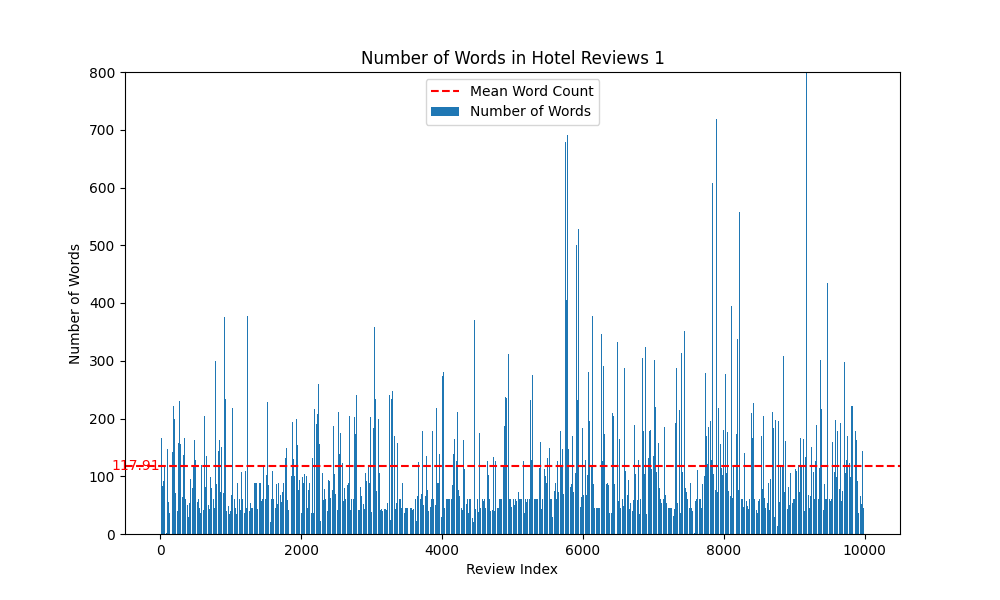
\includegraphics[width=\linewidth]{imgs/word_count_1.png}
  \caption{Average words per review in Datafiniti's Hotel Reviews dataset}
  \label{fig:reviewWords1}
\end{figure}

%% Figure 10
\begin{figure}[H]
  \centering
  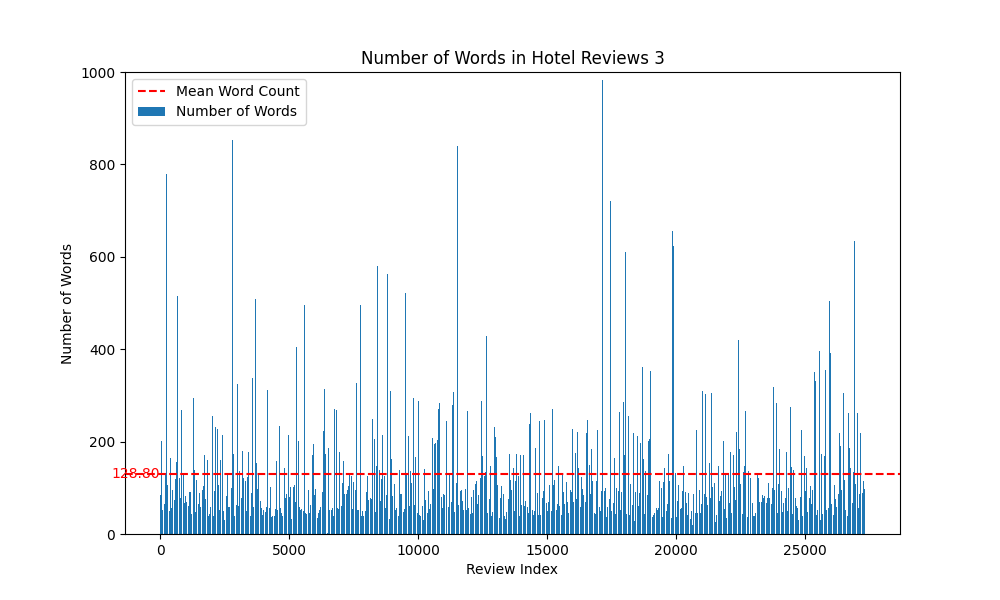
\includegraphics[width=\linewidth]{imgs/word_count_3.png}
  \caption{Average words per review in London Hotel Reviews dataset}
  \label{fig:reviewWords3}
\end{figure}


\begin{figure}[H]
  \centering
  \includegraphics[width=0.8\linewidth]{imgs/q1-p-r-curve-simple.png}
  \caption{Q1 Precision-recall curve using simple system}
  \label{fig:q1_simple}
\end{figure}

\begin{figure}[H]
  \centering
  \includegraphics[width=0.8\linewidth]{imgs/q1-p-r-curve-boosted.png}
  \caption{Q1 Precision-recall curve using boosted system}
  \label{fig:q1_boosted}
\end{figure}


\begin{figure}[H]
  \centering
  \includegraphics[width=0.8\linewidth]{imgs/q2-p-r-curve-simple.png}
  \caption{Q2 Precision-recall curve using simple system}
  \label{fig:q2_simple}
\end{figure}

\begin{figure}[H]
  \centering
  \includegraphics[width=0.8\linewidth]{imgs/q2-p-r-curve-boosted.png}
  \caption{Q2 Precision-recall curve using boosted system}
  \label{fig:q2_boosted}
\end{figure}

\begin{figure}[H]
  \centering
  \includegraphics[width=0.8\linewidth]{imgs/q3-p-r-curve-simple.png}
  \caption{Q3 Precision-recall curve using simple system}
  \label{fig:q3_simple}
\end{figure}

\begin{figure}[H]
  \centering
  \includegraphics[width=0.8\linewidth]{imgs/q3-p-r-curve-boosted.png}
  \caption{Q3 Precision-recall curve using boosted system}
  \label{fig:q3_boosted}
\end{figure}

\begin{figure}[H]
  \centering
  \includegraphics[width=0.8\linewidth]{imgs/q4-p-r-curve-simple.png}
  \caption{Q4 Precision-recall curve using simple system}
  \label{fig:q4_simple}
\end{figure}

\begin{figure}[H]
  \centering
  \includegraphics[width=0.8\linewidth]{imgs/q4-p-r-curve-boosted.png}
  \caption{Q4 Precision-recall curve using boosted system}
  \label{fig:q4_boosted}
\end{figure}

\begin{table}[ht]
\caption{Relevance results for Stopwords Evaluation}
\label{tab:stopwords_results}
\centering
\resizebox{\columnwidth}{!}{
\begin{tabular}{ccccccccc}
\multirow{2}{*}{\textbf{Rank}} & \multicolumn{2}{c}{\textbf{Relevance Q5}} & \multicolumn{2}{c}{\textbf{Relevance Q6}} & \multicolumn{2}{c}{\textbf{Relevance Q7}}\\
 & \textbf{Boosted} & \textbf{Stopwords} & \textbf{Boosted} & \textbf{Stopwords} & \textbf{Boosted} & \textbf{Stopwords}\\
1 & 1 & 1 & 1 & 1 & 0 & 1 \\
2 & 1 & 1 & 1 & 1 & 0 & 1 \\
3 & 1 & 1 & 0 & 0 & 0 & 1 \\
4 & 1 & 1 & 1 & 1 & 0 & 1 \\
5 & 1 & 1 & 0 & 1 & 0 & 0 \\
6 & 1 & 0 & 1 & 0 & 0 & 0 \\
7 & 0 & 1 & 0 & 0 & 0 & 1 \\
8 & 1 & 1 & 0 & 0 & 0 & 0 \\
9 & 1 & 0 & 0 & 0 & 0 & 1 \\
10 & 1 & 1 & 0 & 0 & 0 & 1 \\
11 & 0 & 0 & 0 & 1 & 0 & 1 \\
12 & 0 & 1 & 1 & 1 & 0 & 0 \\
13 & 1 & 1 & 0 & 0 & 0 & 0 \\
14 & 1 & 1 & 0 & 1 & 0 & 1 \\
15 & 1 & 1 & 1 & 1 & 0 & 1 \\
16 & 0 & 1 & 1 & 0 & 0 & 1 \\
17 & 1 & 0 & 1 & 1 & 0 & 1 \\
18 & 1 & 1 & 1 & 0 & 0 & 1 \\
19 & 1 & 1 & 1 & 1 & 0 & 0 \\
20 & 1 & 1 & 0 & 1 & 0 & 0
\end{tabular}
}
\end{table}


\begin{table}[ht]
\caption{Relevance results for initial system evaluation}
\label{tab:raw_results}
\centering
\resizebox{\columnwidth}{!}{
\begin{tabular}{ccccccccc}
\multirow{2}{*}{\textbf{Rank}} & \multicolumn{2}{c}{\textbf{Relevance Q1}} & \multicolumn{2}{c}{\textbf{Relevance Q2}} & \multicolumn{2}{c}{\textbf{Relevance Q3}} & \multicolumn{2}{c}{\textbf{Relevance Q4}} \\
 & \textbf{Simple} & \textbf{Boosted} & \textbf{Simple} & \textbf{Boosted} & \textbf{Simple} & \textbf{Boosted} & \textbf{Simple} & \textbf{Boosted} \\
1 & 1 & 1 & 1 & 1 & 1 & 0 & 1 & 1 \\
2 & 1 & 1 & 1 & 1 & 0 & 1 & 1 & 1 \\
3 & 1 & 1 & 0 & 1 & 1 & 0 & 0 & 0 \\
4 & 1 & 1 & 0 & 1 & 0 & 1 & 0 & 1 \\
5 & 1 & 0 & 1 & 1 & 0 & 0 & 1 & 0 \\
6 & 1 & 1 & 1 & 1 & 1 & 0 & 0 & 1 \\
7 & 1 & 1 & 1 & 0 & 1 & 1 & 0 & 0 \\
8 & 1 & 1 & 1 & 1 & 0 & 0 & 1 & 0 \\
9 & 0 & 1 & 0 & 1 & 1 & 0 & 0 & 0 \\
10 & 0 & 1 & 1 & 1 & 0 & 1 & 1 & 0 \\
11 & 1 & 1 & 1 & 0 & 1 & 1 & 0 & 0 \\
12 & 0 & 1 & 1 & 0 & 1 & 1 & 0 & 1 \\
13 & 0 & 1 & 1 & 1 & 1 & 1 & 0 & 0 \\
14 & 1 & 0 & 1 & 1 & 0 & 1 & 1 & 0 \\
15 & 0 & 1 & 1 & 1 & 1 & 1 & 0 & 1 \\
16 & 0 & 1 & 1 & 0 & 0 & 1 & 0 & 1 \\
17 & 1 & 1 & 1 & 1 & 0 & 0 & 0 & 1 \\
18 & 0 & 1 & 1 & 1 & 0 & 1 & 0 & 1 \\
19 & 0 & 1 & 0 & 1 & 0 & 1 & 1 & 1 \\
20 & 1 & 1 & 1 & 1 & 1 & 1 & 0 & 0
\end{tabular}
}
\end{table}


\end{document}
\endinput
%%
%% End of file `sample-sigconf.tex'.
o